%******************************************************************************************************
%******************************* Third Chapter ********************************************************
%******************************************************************************************************

% Include other chapters so that cross-referencing chapters works nicely.
\externaldocument{{../Chapter1/chapter1}}
\externaldocument{{../Chapter2/chapter2}}
\externaldocument{{../Chapter4/chapter4}}
\externaldocument{{../Chapter5/chapter5}}

% **************************** Define Graphics Path **************************
\graphicspath{{Chapter3/Figs/}}

%******************************************************************************************************
%******************************************************************************************************
%******************************************************************************************************
%******************************************************************************************************
\chapter{Task One: Path Planning}
\label{task1}

In this report the practical work has been clearly divided into two distinct tasks, allowing us to simplify, shorten, and better organise both the work and the reporting of it. This chapter of the report will discuss the first of the two practical tasks, covering the design, implementation, and testing of the solution for the path planning problem discussed in Section \ref{intro:objectives}.

%******************************************************************************************************
%******************************************************************************************************
\section{Path Planning - Aims}
\label{task1:aims}

This section of work is aimed at producing a system to enable us to both plan and define paths for the UAV to follow. The paths we need to produce must in fact be sections of larger mission plans, and must be used to enable the UAV to travel between the end of one imaging path and the start of the next. Stock ArduPlane can of course offer this, but what it cannot offer is the abilty to ensure the UAV is aligned with the imaging path before beginning to travel along it. This, in essence, is the simplest definition for this task; to define flight paths that enable the UAV to correctly align itself with a given imaging path prior to starting it.  

Fig. \ref{fig:baseArduPlane} shows the results of a simulated flight using the stock, currently released version of ArduPlane. The mission for this simulation was planned to give an idea of how ArduPlane performs at the moment, and how its current waypoint navigation system does not enable us to align with imaging paths. If we imagine that the three vertically aligned paths between waypoints 2 and 3, 4 and 5, and 6 and 7 are imaging paths, we can clearly see that our UAV would be missing considerable sections of these important paths. The result of this would be that the images captured may entirely miss areas of land towards the beginning of these paths. 

Currently in ArduPlane, the only way to ensure our UAV is aligned with an imaging path to make sure we are able to photograph all of the ground beneath an imaging path is to add additional waypoints. Fig. \ref{fig:waypoingmanipulation} shows how this would work. A waypoint is added as a form of extension to the first imaging path before the UAV travels the second imaging path, helping the UAV turn in time. Although this does work, it adds complexity and increases the time taken to plan an effective imaging run. One of our primary motivations for this project is to improve the path planning experience, by ensuring the UAV flies where we want it to without additional hassle. As such this is simply not an acceptable solution to the problem, so we must implement one ourselves.

\begin{figure}[htbp!] 
\centering    
\includegraphics[width=0.8\textwidth]{BaseArduPlane}
\caption[Stock ArduPlane Path Tracking]{Results of a flight simulation using stock ArduPlane}
\label{fig:baseArduPlane}
\end{figure}

\begin{figure}[htbp!] 
\centering    
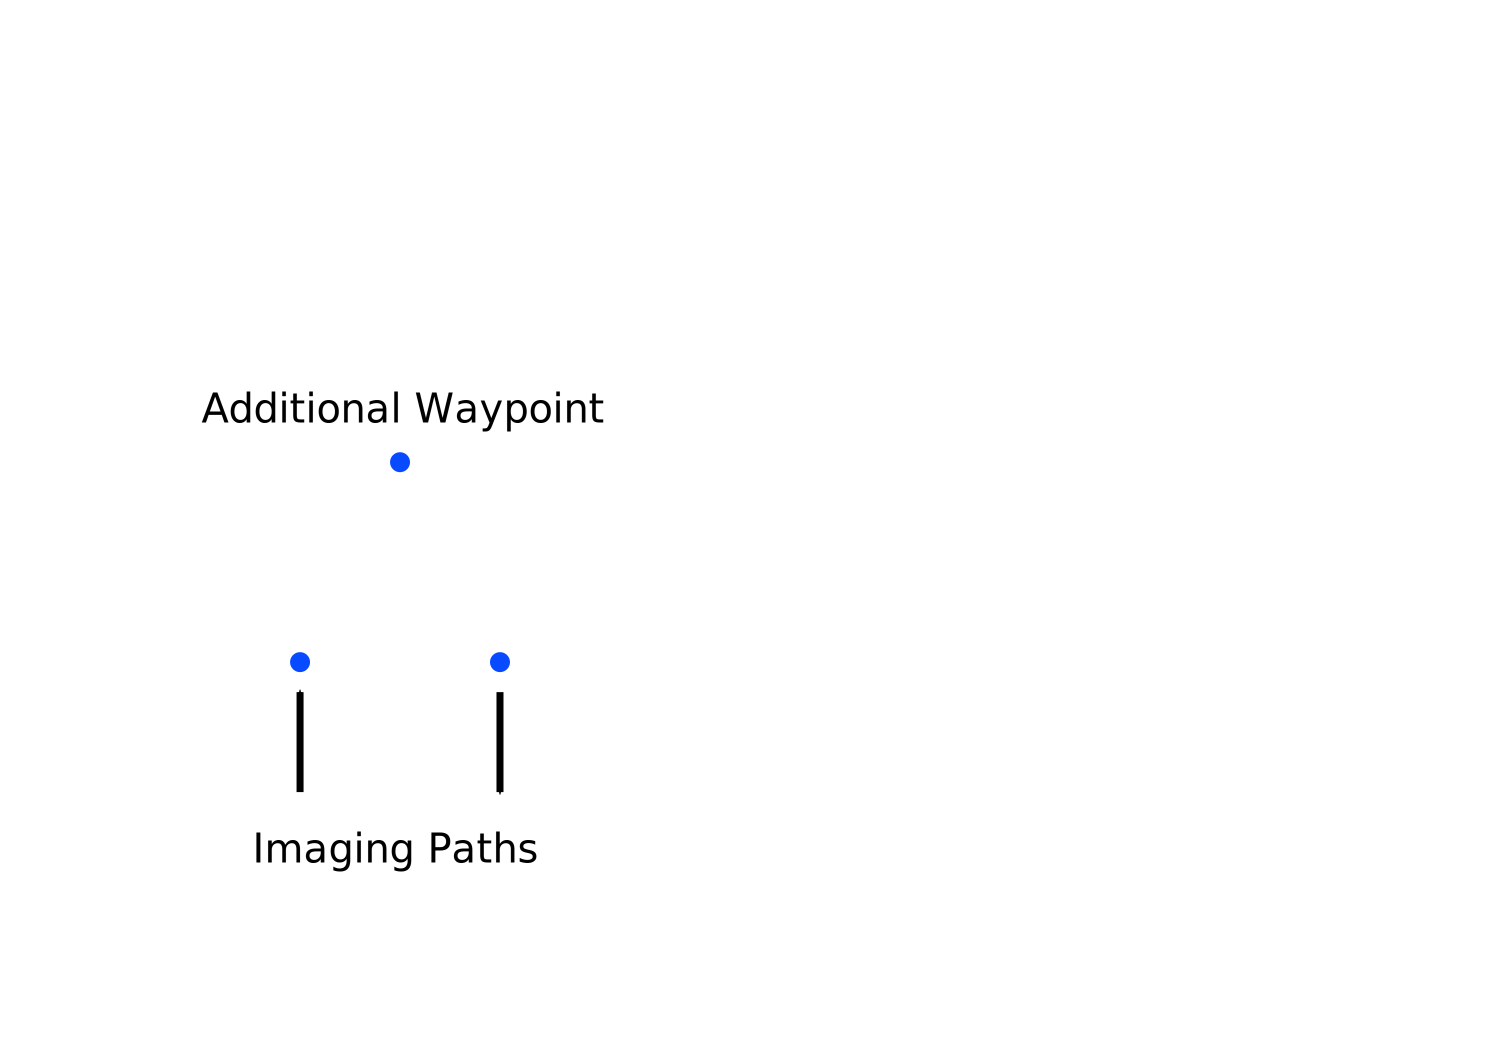
\includegraphics[width=0.4\textwidth]{WaypointManipulation}
\caption[Aligning With an Imaging Path in Stock ArduPlane]{One solution for aligning with an imaging path in the current version of ArduPlane via waypoint manipulation}
\label{fig:waypoingmanipulation}
\end{figure}

One of the problems we have is that ArduPlane navigates via straight lines drawn between points and has no concept of pre-emptive flight control or prioritisation of path sections. We can utilise Dubins paths as described in Section \ref{litrev:dubins} to decribe the shortest path possible between imaging paths that take the orientation of the UAV into consideration. We can then extend this work using the research discussed in Section \ref{litrev:path} to also handle the effects of wind on navigation. Using these techniques, we can introduce extra navigation steps at the planning stage that will in effect prioritise our imaging paths by ensuring the UAV arrives at the start of the path with the correction orientation and direction of travel. If a solution were to be implemented into the mission planning software, it would enable the user to specify the start and end points of imaging runs, and automatically calculate the desired Dubins path between them. 

As mentioned in Section \ref{intro}, this project is being run in parallel with another project investigating a related area of work. This other project is interested in path optimisation, for which one important feature is of course length. It was decided that this optimisation research should utilise the results of this work when calculating path lengths, suggesting the integration of the two projects at a later date. The result of this is that an additional aim for this task is to be able to share the system generated here for use in other work. It was decided that the best way to do this would be to create a standalone console application that could be compiled and shared, which took a number of parameters and returned details about the resulting paths. This shall be discussed further along with the other implementation work.

In effect we aim to introduce a new turning technique to the autopilot system, and the first stage of completing this is to be able to plan paths that define these turns. The result of this work will be effectively replacing the straight lines currently joining the ends of imaging paths with curved turns in the form of Dubins paths. We place no importance on the route travelled between the imaging paths, so we can replace the current paths with our own in order to prioritise aligning with imaging paths. By utilising Dubins paths we will also be improving battery life, as by their very definition DUbins paths are the shortest suitable routes we can take. 

We can summarise our aims for this task as covering the following points

\begin{itemize}
	\item Being able to calculate suitable Dubins paths for a given UAV platform, taking into consideration its turning radius
	\item Being able to calculate suitable Dubins paths for a given UAV platform flying in a given wind condition
	\item Being able to define the resulting Dubins paths segments, either via location or length
	\item Allowing a user to specify a start and end point with prescribed orientation for our Dubins paths in all scenarios
	\item Creating a standalone application to share the results of this work
\end{itemize}

%TODO finalise aims
%******************************************************************************************************
%******************************************************************************************************
\section{Path Planning - Design and Planning}
\label{task1:design}

As we can infer from the aims above, this task needed to be completed in a number of steps. To achieve this, the overall path planning tasks was split up into a number of sub-tasks, the order in which these were carried out is as follows:

\begin{enumerate}
	\item Plot Dubins paths in MATLAB
	\item Plot the effect of a given wind input on the ground relative plot of the same Dubins paths
	\item Implement a system to select an air relative Dubins path that results in the ground relative path tracking to our desired location and orientation
	\item Implement this system as a standalone console application
\end{enumerate}

Throughout all stages of this task it was important to test the completed work to ensure we were prepared to move onto the next subtask. This was also important so as to minimise the risk of carrying bugs and errors forward throughout the project. As such there were testing steps carried out at for all sub-tasks, and these shall be documented in Section \ref{task1:testing}. 

\subsection{Sub-Task 1: Plotting Dubins Paths in MATLAB}
\label{task1:design:subtask1}

The design process for this task was very simple, as the author was aware of the availability of the C based Dubins path application and associated MATLAB wrapper \cite{WalkerDubinsCurves,MexDubinsCurves}. From the start the author was aware of the risk of using unverified work, however by analysing the source code and comparing the mathematical calculations with those found in \cite{shkel2001classification}, it was deemed suitable to progress using these resources. After this analysis of the supplied code, the only work left in order to complete this sub-task would be to supply inputs to the Dubins application, process outputs, and plot the results.

Throughout this sub-task we need to ensure that we are able to supply any combination of inputs to the program, specifying locations and orientations for both ends of the Dubins path as well as turning radius for our UAV.

\subsection{Sub-Task 2: Plotting the Effects of Wind on Dubins Paths}
\label{task1:design:subtask2}

The next step for us to calculate the ground relative path followed by the UAV when commanded to fly a Dubins path in a wind condition. Regarding the air relative frame of reference, the UAV will be simply flying a Dubins path, however if we were to examine the GPS location data we would instead be seeing the UAV having flown a different path entirely. This sub-task is designed to be completed in MATLAB and to extend the capabilities of the program developed in sub-task 1. Alongside the original Dubins path plot we should plot the wind-affected path so as to easily allow comparison between the two. The plot should also display information about the wind vector to help visual inspection of the resulting paths. 


\subsection{Sub-Task 3: Generating an Air Relative Path Based on Desired Ground Relative Destination}
\label{task1:design:subtask3}

This sub-task is where we finalise our new path planning system. For the application of aerial photography, the frame of reference that is most relevant to us is the ground relative frame. We want to be able to command the UAV to a location above a certain point on the ground, not a certain point in air. As such, we to implement a system that takes a desired destination, and calculates the air relative Dubins path. This Dubins path must of course take wind into consideration, as well as UAV orientations at either end of the turn alongside the UAV turning radius. Once again this is to be implemented entirely in MATLAB. 

This will use a similar plot style to that produced in sub-task 2, allowing us to compare air and ground relative paths as well as the wind vector. This will hopefully enable us to quickly spot any glaring errors, as well as do some rudimentary estimations on whether the effect of wind is being calculated correctly.

This system will be heavily based on the research discussed in Section \ref{litrev:path}, implementing the search algorithm as mentioned.

\subsection{Sub-Task 4: Creating a Standalone Console Application}
\label{task1:design:subtask4}

The final step for completing the path planning part of this project is to create the console application. This console application will serve three main purposes; firstly it will form an integral part of path length calculation in the other project relating to this work, mentioned in Section \ref{intro}. Secondly it will enable us to do some fast and thorough testing of our path generation search algorithm, as will be discussed later. Finally, it will be used in the testing stages of the second task in this project, the path following task.

%******************************************************************************************************
%******************************************************************************************************
\section{Path Planning - Implementation}
\label{task1:implementation}

\subsection{Sub-Task 1: Plotting Dubins Paths in MATLAB}
\label{task1:implementation:subtask1}



\subsection{Sub-Task 2: Plotting the Effects of Wind on Dubins Paths}
\label{task1:implementation:subtask2}


\subsection{Sub-Task 3: Generating an Air Relative Path Based on Desired Ground Relative Destination}
\label{task1:implementation:subtask3}


\subsection{Sub-Task 4: Creating a Standalone Console Application}
\label{task1:implementation:subtask4}

%******************************************************************************************************
%******************************************************************************************************
\section{Path Planning - Testing}
\label{task1:testing}

\subsection{Sub-Task 1: Plotting Dubins Paths in MATLAB}
\label{task1:testing:subtask1}


\subsection{Sub-Task 2: Plotting the Effects of Wind on Dubins Paths}
\label{task1:testing:subtask2}


\subsection{Sub-Task 3: Generating an Air Relative Path Based on Desired Ground Relative Destination}
\label{task1:testing:subtask3}


\subsection{Sub-Task 4: Creating a Standalone Console Application}
\label{task1:testing:subtask4}
